%!TEX root = ../../../adrien_gomar_phd.tex
\chapter{Contra-rotating open rotors}
\label{cha:cror}

\chabstract{In this chapter, we first recall the thrust
and propulsive efficiency equations. Using these equations,
the propeller engines are shown to be good candidates
for efficient engines, mainly due to its high bypass ratio.
The geometry, general principle, similarity coefficients
and main physical phenomena of such engines are 
highlighted. In addition to that, it is shown that even if efficient,
the propeller engines suffer from a residual swirl motion.
To tackle this problem, the contra-rotating open rotor
technology is presented as long with its main source of unsteadiness.
The challenges associated to this engine are finally detailed
and we show that aeroelasticity needs to be accounted for.}

\minitoc
\newpage

\section{Generalities of propulsion}
\label{sec:cror_intro}
%!TEX root = ../../../adrien_gomar_phd.tex

For an aircraft in steady flight conditions, 
lift balances weight and 
thrust balances drag. This explains why engineers try
indefinitely to reduce weight while increasing
thrust. A trade-off between those two is to work
on the propulsive efficiency of the engine. In this
section, general information on propulsion
that leads to the concepts of propeller and
contra-rotating open rotor are given.

\subsection{Thrust equation}
\label{sub:cror_thrust}
Consider the conservative equation of momentum
\begin{equation}
	\frac{\partial \rho \vec{V}}{\partial t} 
	+ \nabla \cdot (\rho \vec{V} \otimes \vec{V} + p \mathbb{I} - \vec{\vec{\Sigma}}_v) = 0,
\end{equation}
where $\rho$ is the density, $\vec{V}$ the velocity vector, $p$ the pressure and
$\vec{\vec{\Sigma}}_v$ the viscous stress terms.
Consider two closed domains $\Sigma$ and $\Sigma^\prime$ as
shown in Figure~\ref{fig:cror_control_volume}.
\begin{figure}[htp]
  \centering
  \includegraphics*[width=0.30\textwidth]{control_volume.pdf}
  \caption{Domains used for the application of the momentum equation.}
  \label{fig:cror_control_volume}
\end{figure}
The domain $\Sigma^\prime$ represents a fluid domain outside from the
engine encompassed by the solid domain $\Sigma$.
Taking a steady state hypothesis, one can write
\begin{equation}
	\oint_{\Sigma} \left(\rho \vec{V} \otimes \vec{V} + 
	                       p \mathbb{I} - 
	                       \vec{\vec{\Sigma}}_v \right) \cdot \vec{n} \diff S
    =
   	\oint_{\Sigma^\prime} \left(\rho \vec{V} \otimes \vec{V} + 
	                       p \mathbb{I} - 
	                       \vec{\vec{\Sigma}}_v \right) \cdot \vec{n} \diff S,
\end{equation} 
where $\vec{n}$ is the normal vector.
As $\Sigma^\prime$ is an arbitrary domain, we can take it sufficiently
away from the engine so that $\vec{\vec{\Sigma}}_v$ becomes zero (\emph{i.e.}
viscosity stress terms are null).
Moreover, 
\begin{equation}
	\oint_{\Sigma} \left(\rho \vec{V} \otimes \vec{V} \right) \cdot \vec{n} \diff S = 0,
\end{equation}
since the surface is solid ($\vec{V} = \vec{0}$ on wall). 
If $\vec{F}$ denotes the resultant forces acting on $\Sigma$
\begin{equation}
	\vec{F} = \oint_{\Sigma} \left(p \mathbb{I} - 
	\vec{\vec{\Sigma}}_v \right) \cdot \vec{n} \diff S,
\end{equation}
then
\begin{equation}
	\vec{F} = \oint_{\Sigma^\prime} \left(\rho \vec{V} \otimes \vec{V} +
	p \mathbb{I} \right) \cdot \vec{n} \diff S.
\end{equation}
Assuming that $\Sigma^\prime$ is a stream tube, and projecting the equation
onto the $x$-axis gives the formula for the thrust $F_x$
\begin{equation}
	F_x = \dot{m} V_{out} + p_{out} S_{out}
	- \dot{m} V_{in} - p_{in} S_{in},
\end{equation}
using the notation of Figure~\ref{fig:cror_control_volume}.

Far downstream of the engine $S_{in} = S_{out}$ and
considering that we have an adapted nozzle ($p_{in} = p_{out}$),
the thrust $F_x$ can be written as
\begin{equation}
	\fbox{$
	F_x = \dot{m} (V_{out} - V_{in}) = \dot{m} \Delta V_x
	$}
	\label{eq:cror_thrust}
\end{equation}
where $\dot{m}$ is the mass-flow rate going through the
propeller and $\Delta V_x$ is
the increment of axial velocity. From this simple equation,
one can see that to increase the thrust $F_x$, there are two parameters:
the mass-flow and the axial velocity increment.

\subsection{Global propulsive efficiency}
\label{sub:cror_efficiency}

The global propulsive efficiency $\eta$ measures the 
success in converting a mechanical power into a
propulsive power. It results from the combination
of the kinetic efficiency $\eta_{K}$ and the propulsive efficiency
$\eta_{PR}$
\begin{equation}
	\eta = \eta_{K} \times \eta_{PR}.
\end{equation}
This is schematically represented in Figure~\ref{fig:cror_efficiency}.
\begin{figure}[htp]
  \centering
  \includegraphics*[width=0.40\textwidth]{efficiency.pdf}
  \caption{Efficiency relations from mechanical power to propulsive power.}
  \label{fig:cror_efficiency}
\end{figure}

\paragraph{Kinetic efficiency}
The kinetic efficiency measures the success in converting the mechanical
power $P_m$ into a kinetic power $P_k$
\begin{equation}
	\eta_K = \frac{P_k}{P_m}.
\end{equation}

The mechanical power delivered as input
can be computed through the first thermodynamic principle. In fact, in absence
of heat exchange, the mechanical power $P_m$ can be estimated as
\begin{equation}
	P_m = \dot{m} (h_{i_{out}} - h_{i_{in}}),
\end{equation}
where $h_i$ is the total enthalpy and subscript $in$ and $out$ are
the input and output, respectively, of the propulsion system as represented
in Figure~\ref{fig:cror_control_volume}.
The kinetic power $P_k$ is given by
\begin{equation}
	P_k = \dot{m} \left(\frac{1}{2} V^2_{out} -
	\frac{1}{2} V^2_{in} \right).
\end{equation}
This leads to a kinetic efficiency that can be expressed as
\begin{equation}
	\eta_{K} = \frac{V^2_{out} - V^2_{in}}{2 (h_{i_{out}} - h_{i_{in}})}
\end{equation}

\paragraph{Propulsive efficiency}
The propulsive efficiency $\eta_{PR}$ measures the success
in creating a propulsive power $P_{pr}$ from a
kinetic power $P_k$
\begin{equation}
	\eta_{PR} = \frac{P_{pr}}{P_k}.
\end{equation}
The propulsive power is computed using the thrust $F_x$
\begin{equation}
	P_{pr} = F_x \times V_{\infty},
\end{equation}
where $V_{\infty}$ is the free-stream velocity.
Finally, if the free-stream velocity is the inlet velocity $V_{in}$
and the inlet and outlet velocities are purely axial
\begin{equation}
	\fbox{$
	\eta_{PR} = \displaystyle \frac{1}{1 + \frac{V_{out} - V_{in}}{2 V_{in}}}
	$}
	\label{eq:cror_propulsive_efficiency}
\end{equation}
This formula means that the most efficient engine produces
a very small velocity increment.

\subsection{Toward propeller engines}
\label{sub:cror_toward_propeller}

One way to improve the environmental footprint of
airplanes engines is to increase the propulsive efficiency
by reducing the kinetic power needed to drive the engine.
Doing so while maintaining the thrust can be achieved through
a higher mass-flow rate. Two new concepts are thus derived from
this simple statement: the High ByPass-Ratio (HBPR) which
is basically a turbofan with a larger fan exhaust, and the
propeller whose mass-flow rate is not limited
by the architecture, as the blades are not within a nacelle.
In the following section, the propeller engine will be detailed
and the drawbacks of such an architecture will be highlighted to
motivate the use
of a second propeller row, yielding the contra-rotating open rotor
architecture.




\section{Propeller}
\label{sec:cror_propeller}
%!TEX root = ../../../adrien_gomar_phd.tex

\subsection{Geometry}
\label{sub:cror_propeller_geometry}

A propeller is composed of a hub and a rotating set of 
$B$ blades as schematically represented in
Fig.~\ref{fig:cror_propeller_geometry}. The hub
is the part on which the blades are mounted.
We set the diameter of these blades being $D$
and their rotation speed being $\Omega$. 
In front of the propeller, there is a spinner which is
a conic geometry element that helps
smoothing the inflow for the propeller blades.
The propeller can be seen as
a turbofan whose fan is not within a nacelle.
\begin{figure}[htb]
  \centering
  \includegraphics*[scale=0.30]{propeller_geometry.pdf}
  \caption{Geometry of a propeller.}
  \label{fig:cror_propeller_geometry}
\end{figure}
Its absence implies that theoretically, the mass-flow can be
infinite. To quantify this, it is common for engines to
consider the bypass ratio. It is defined as the ratio between the
cold air (the un-combustioned air)
divided by the hot air (the air that goes through the engine core).
To give an idea, one of the highest bypass ratio engine on today's aircraft is given
by the Pratt~\&~Whitney~PW1000G and is~12, while propellers are estimated
to have a bypass ratio of~50. 
This number is representative of the mass-flow rate generated by the engine.
However, we have seen that mass-flow is a parameter that can be used to increase
the thrust so as the velocity difference. Assuming that in a classical ducted turbofan, 
the bypass ratio is limited to~12, the only
way to increase the thrust is to increase the 
velocity which deteriorates the propulsive efficiency. In absence of a duct,
no limitation is set by the nacelle on the mass-flow rate.
This explains why this architecture has
regained interest. However, propellers
have been limited to low Mach number flight condition
due to the high relative velocity seen at the tip of the blades.

\subsection{Velocity triangle}
\label{sub:cror_propeller_velocity_triangle}
The velocity triangle applied to a propeller configuration
is shown in Fig.~\ref{fig:cror_velocity_triangle_propeller}.
The aim of a propeller is to create thrust through an increase
of the axial velocity noted $\Delta V_x$ in the diagram. To do
so, the relative flow field is straighten up. This gives both
an increase in axial velocity but also in tangential velocity.
In fact, the inflow that was purely axial has a tangential
component at the outlet. This is called the swirl and
is a lost energy as it cannot be used to produce thrust.
\begin{figure}[htbp]
  \centering
  \includegraphics*[scale=0.40]{velocity_triangle_propeller.pdf}
  \caption{Velocity triangle applied to a propeller.}
  \label{fig:cror_velocity_triangle_propeller}
\end{figure}
Moreover, the relative velocity $W$ should be kept subsonic
otherwise the propulsive efficiency is reduced. This limits
the free-stream velocity $V_0$ of the aircraft and the size of 
the propeller as $U = \Omega R$.

\subsection{Similarity coefficients}
\label{sub:similarity_coefficients}
To evaluate the performances of the propeller, four similarity
coefficients are commonly used:
the advance ratio $J$ that represents the operating point of the propeller,
the thrust $C_t$ and power $C_p$ coefficients that estimate its performance and finally
the efficiency $\eta$:
\begin{equation}
    J = \frac{V_0}{n D}, \quad
    C_T = \frac{F_x}{\rho n ^ 2  D ^ 4}, \quad
    C_P = \frac{M_x \Omega}{\rho n ^ 3 D ^ 5}, \quad
    \eta = J \frac{C_T}{C_P},
\end{equation}
where $V_0$ is the free-stream velocity 
as shown in Fig.~\ref{fig:cror_propeller_geometry},
$\rho$ the free-stream density,
$n$ the rotation frequency ($n = \Omega / 2 \pi$) and
$M_x$ the axial torque.
The efficiency defined here is the global propulsive efficiency
as it gives the ratio of the propulsive power over the mechanical power.

An estimation of the variation of the advance ratio $J$ and the 
efficiency $\eta$ depending on the flight conditions can be given as follow
\begin{alignat}{4}
    \text{(cruise)} \quad  0.8 &< \eta &< 0.95, \quad 1 &< J < 3.5 \\
    \text{(take-off)} \quad  0.5 &< \eta &< 0.8, \quad J &< 1.
\end{alignat}

\subsection{Main physical phenomena}
\label{sub:cror_propeller_physics}

\begin{figure}[htb]
  \centering
  \subfigure[Wakes]{
      \label{fig:propeller_wakes}
      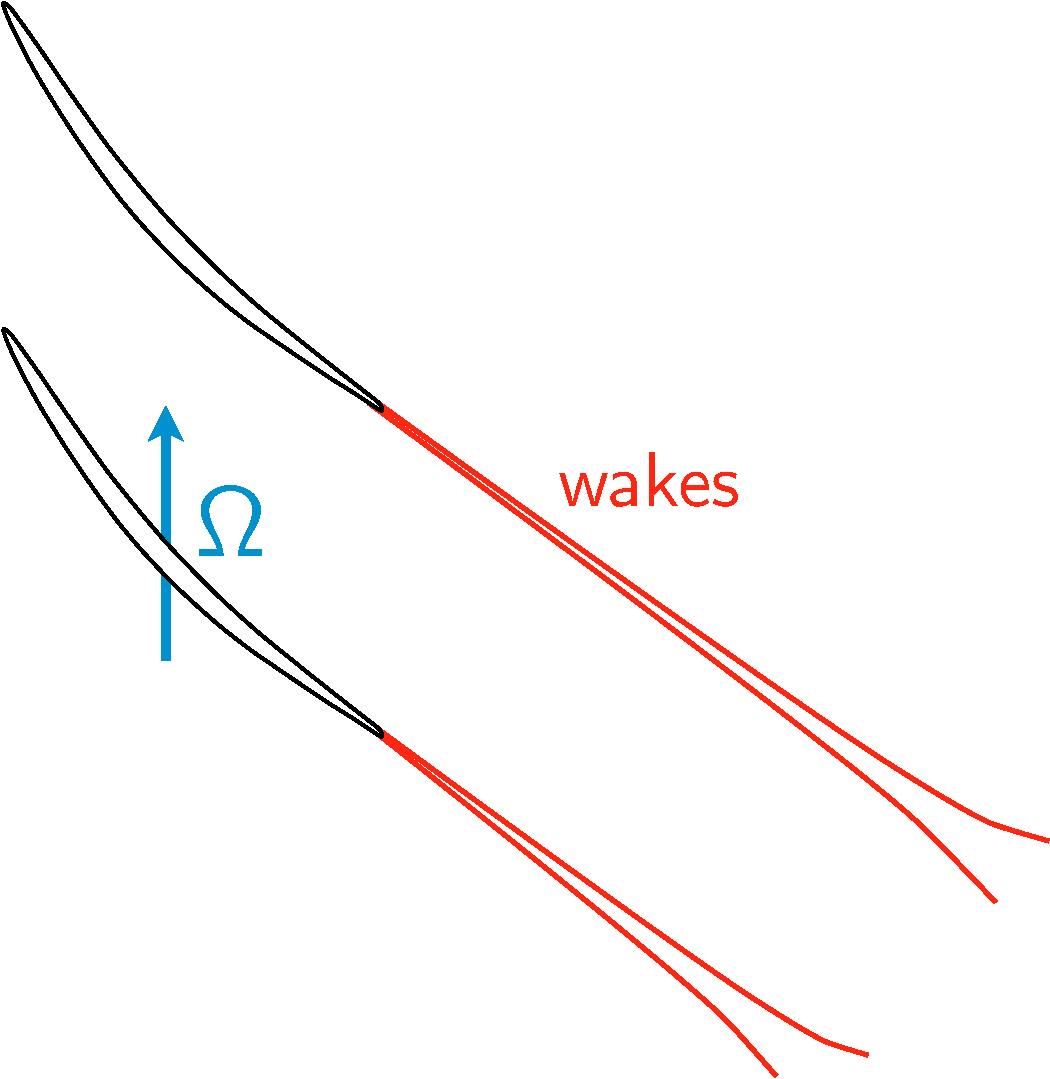
\includegraphics[scale=.2]{propeller_wakes.pdf}}
  \quad\subfigure[Tip vortices]{
      \label{fig:propeller_tip_vortices}
      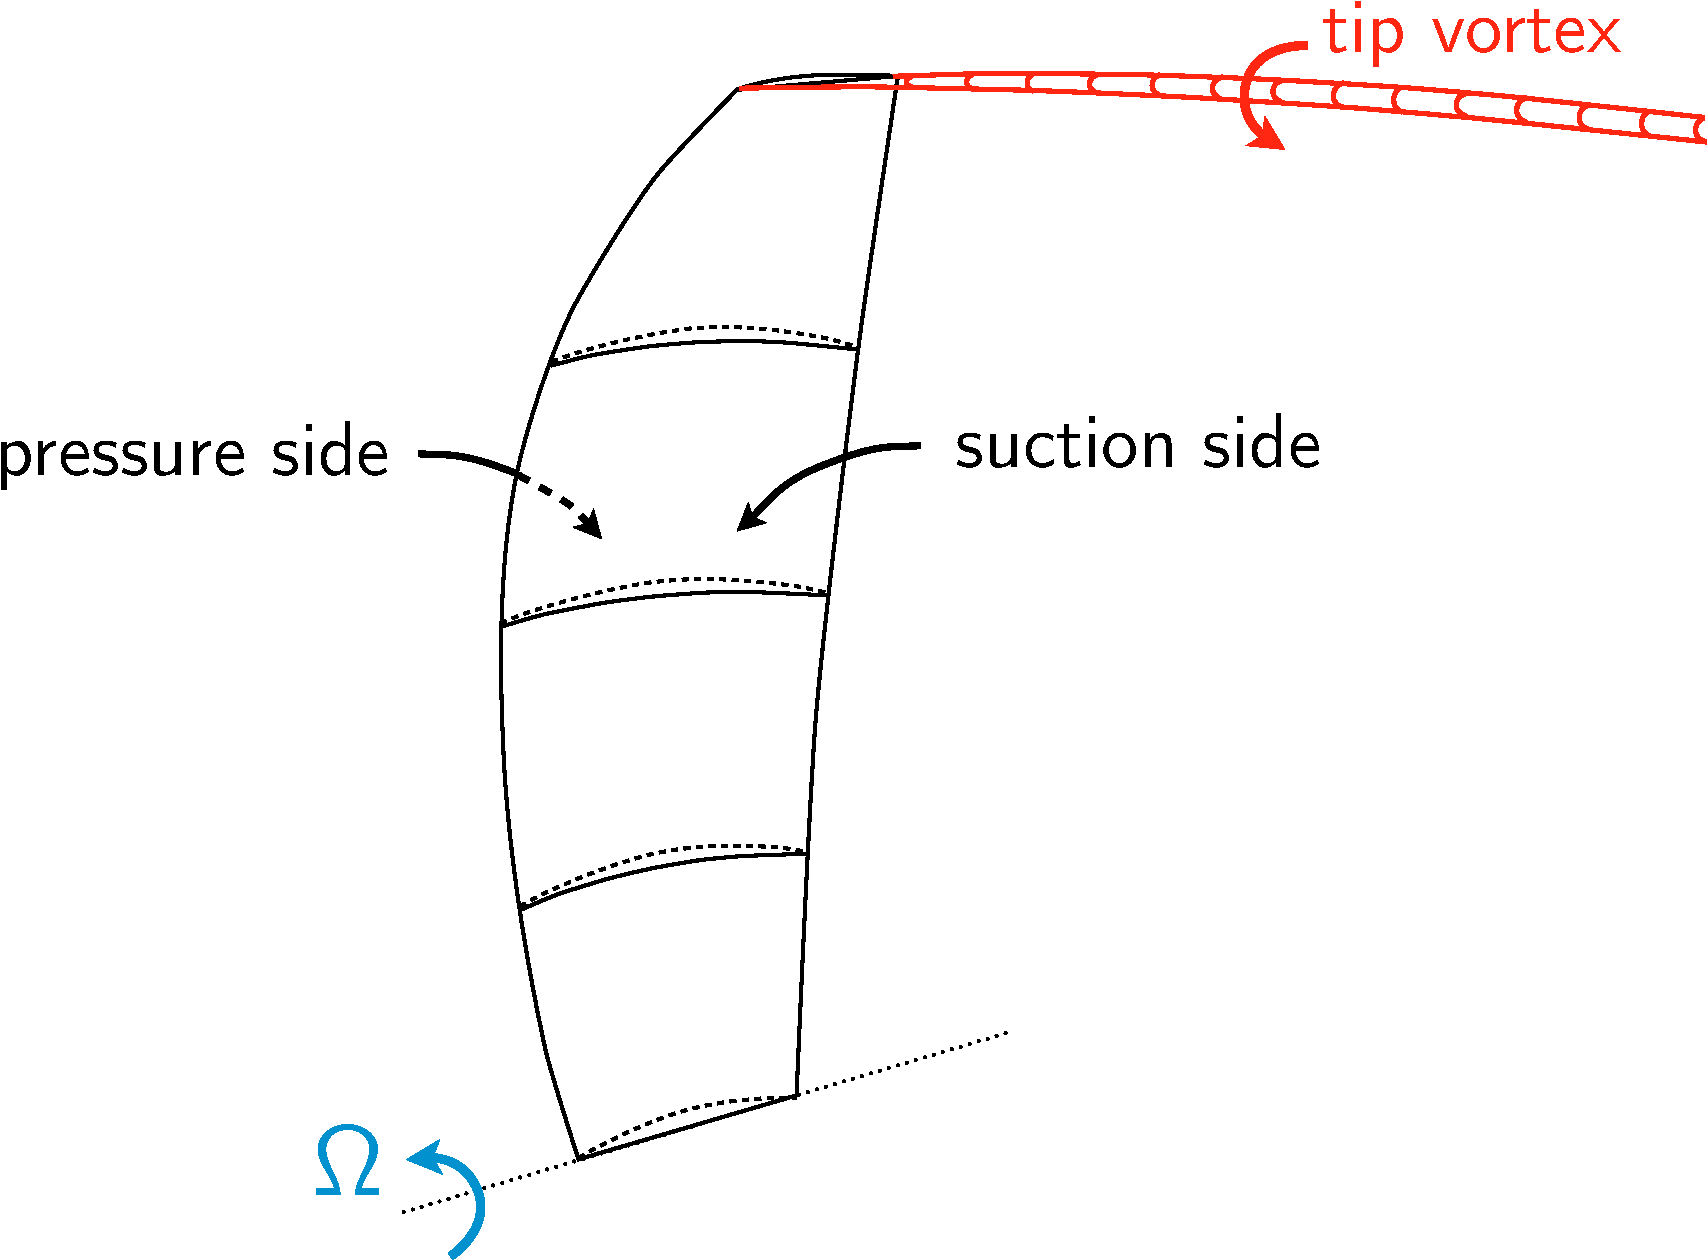
\includegraphics[scale=.2]{propeller_tip_vortices.pdf}}
  \quad\subfigure[Stream tube contraction]{
      \label{fig:propeller_stream_tube}
      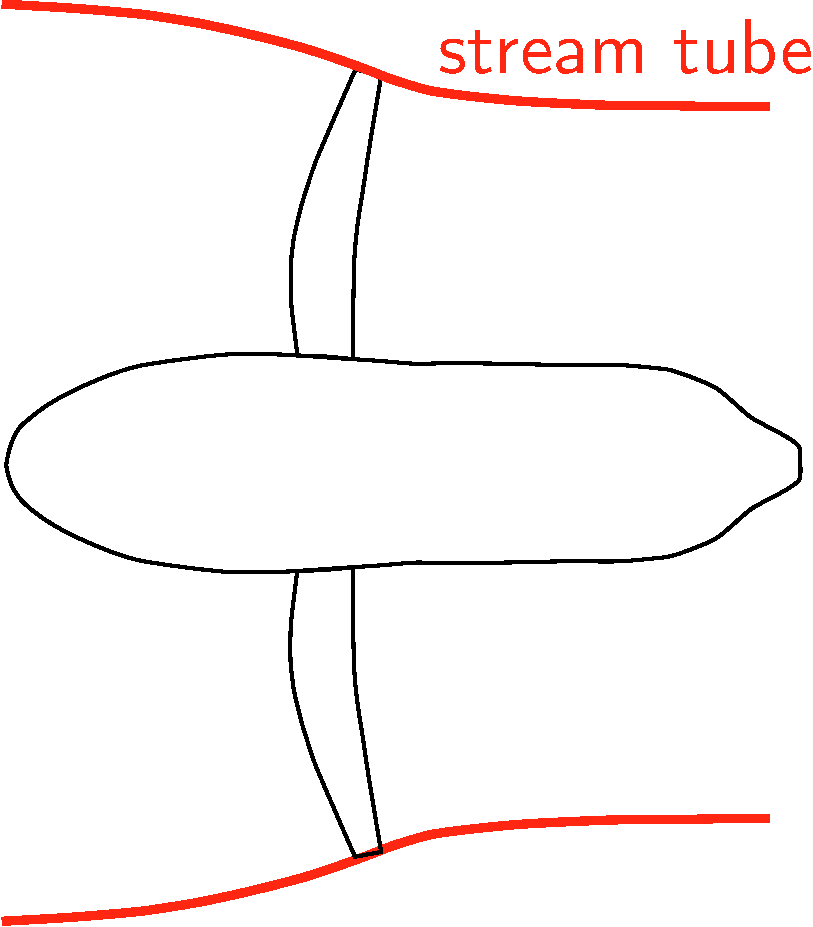
\includegraphics[scale=.2]{propeller_stream_tube.pdf}}
  \caption{Main physical phenomena seen in a propeller.}
  \label{fig:propeller_phys_phenomena}
\end{figure}
The main physical phenomena that can be seen in a propeller are schematically represented
in Fig.~\ref{fig:propeller_phys_phenomena}. Firstly, due to the presence of a boundary
layer on the pressure side and suction side of the blades, a wake is shed behind each blade, which
is represented by a momentum deficit. It is mostly a two-dimensional
phenomenon seen at each radii. Secondly, in the tip region of the blade, the pressure difference between 
the sides of the blade induces a vortex counter-rotating with respect to 
the rotation speed. Their convection is ensured by the local relative velocity giving them
an helical path propagating downstream.
To reduce this phenomenon, one way is to modify the geometry of the tip
of the blades but does not fully annihilate this phenomenon. 
Finally, the propeller generates thrust through an acceleration of the fluid. Thus, the stream
tube is contracted. All of these phenomena are stationary in their relative frame of reference.


\section{Contra-rotating open rotors}
\label{sec:cror_cror}
%!TEX root = ../../../adrien_gomar_phd.tex

As shown above in a single rotor propeller, the outlet velocity is not axial
yielding a residual tangential velocity $\Delta V_{\theta}$,
which forms the swirl. 
This is a lost energy that deteriorates the propulsive efficiency. 
To recover it, a second contra-rotating rotor can be used~\cite{Hager1988}.
We will see in this section through a simple velocity triangle exercise that
the swirl is annulated by the second rotor. This increases the propulsive
efficiency as shown by \citet{Hughes1989} and reported 
in Figure~\ref{fig:hughes_propulsive_efficiency}.
\begin{figure}[htp]
  \centering
  \includegraphics*[width=0.40\textwidth]{hughes_propulsive_efficiency}
  \caption{Benefit of using a contra-rotating open rotor, from \citet{Hughes1989}.}
  \label{fig:hughes_propulsive_efficiency}
\end{figure}

\subsection{Geometry}
\label{sub:cror_geometry}

Figure~\ref{fig:cror_geometry} depicts the main
geometrical parameters of a CROR.
It is composed of two rotors, the first one is called
the front rotor and the second one is called the rear or aft rotor.
Generally, they do not have the same diameter and rotation speed. 
Thus, subscript $f$ and $r$ denotes respectively,
the front and the rear parameters.
The difference of diameter is called the clipping or cropping
of the blades and is evaluated through the non-dimensional parameter
$\kappa$
\begin{equation}
    \kappa = \frac{D_f - D_r}{D_f}.
\end{equation}
By clipping the rear
rotor, tip vortices shed by the front rotor are not likely
to hit the rear rotor blades.
Finally, the spacing between the rotors
is evaluated as the difference between the axial minimum of the
rear blade minus the axial maximum of the front blade. The spacing
is one of the adjustment parameters used to minimize the unsteady
interaction between the rotors to reduce noise. In fact, 
heterogeneities are lessened along with the convection of
the flow field. These heterogeneities are responsible
for the unsteady interactions and, by extrapolating, for noise generation.
\begin{figure}[htp]
  \centering
  \includegraphics*[scale=0.3]{cror_geometry.pdf}
  \caption{Contra-rotating open rotor geometrical parameters.}
  \label{fig:cror_geometry}
\end{figure}

Two types of contra-rotating open rotors have emerged, the
puller CROR whose blades are near the front of the spinner as 
shown in Figure~\ref{fig:cror_configurations}. As the
name indicates, this configuration is mounted in front of the
wing. It is particularly interesting as the blades will see
a uniform flow. However, these all suffer from the same incidence as that
of the wing. This can give large in-plane forces 
(forces normal to the rotation axis~\cite{ThesisFrancois}) compared to pusher
configurations. In opposite, the deflection of the flow due to the wing provides
a smaller incidence.
Moreover, the distortion generated
by the CROR will disturb the flow around the wing. As one way to reduce
consumption of airplanes is to have laminar wings, this configuration
is less studied. The second configuration is the pusher
configuration. It is designed to be mounted on a pylon which will thus
interact with the CROR, but laminar wings might be considered with
this configuration. In this thesis, we will deal with a pusher configuration
in Chapters~\ref{cha:dream_ls_isolated} and
\ref{cha:dream_hs_isolated}.
\begin{figure}[htp]
  \centering
  \subfigure[puller]{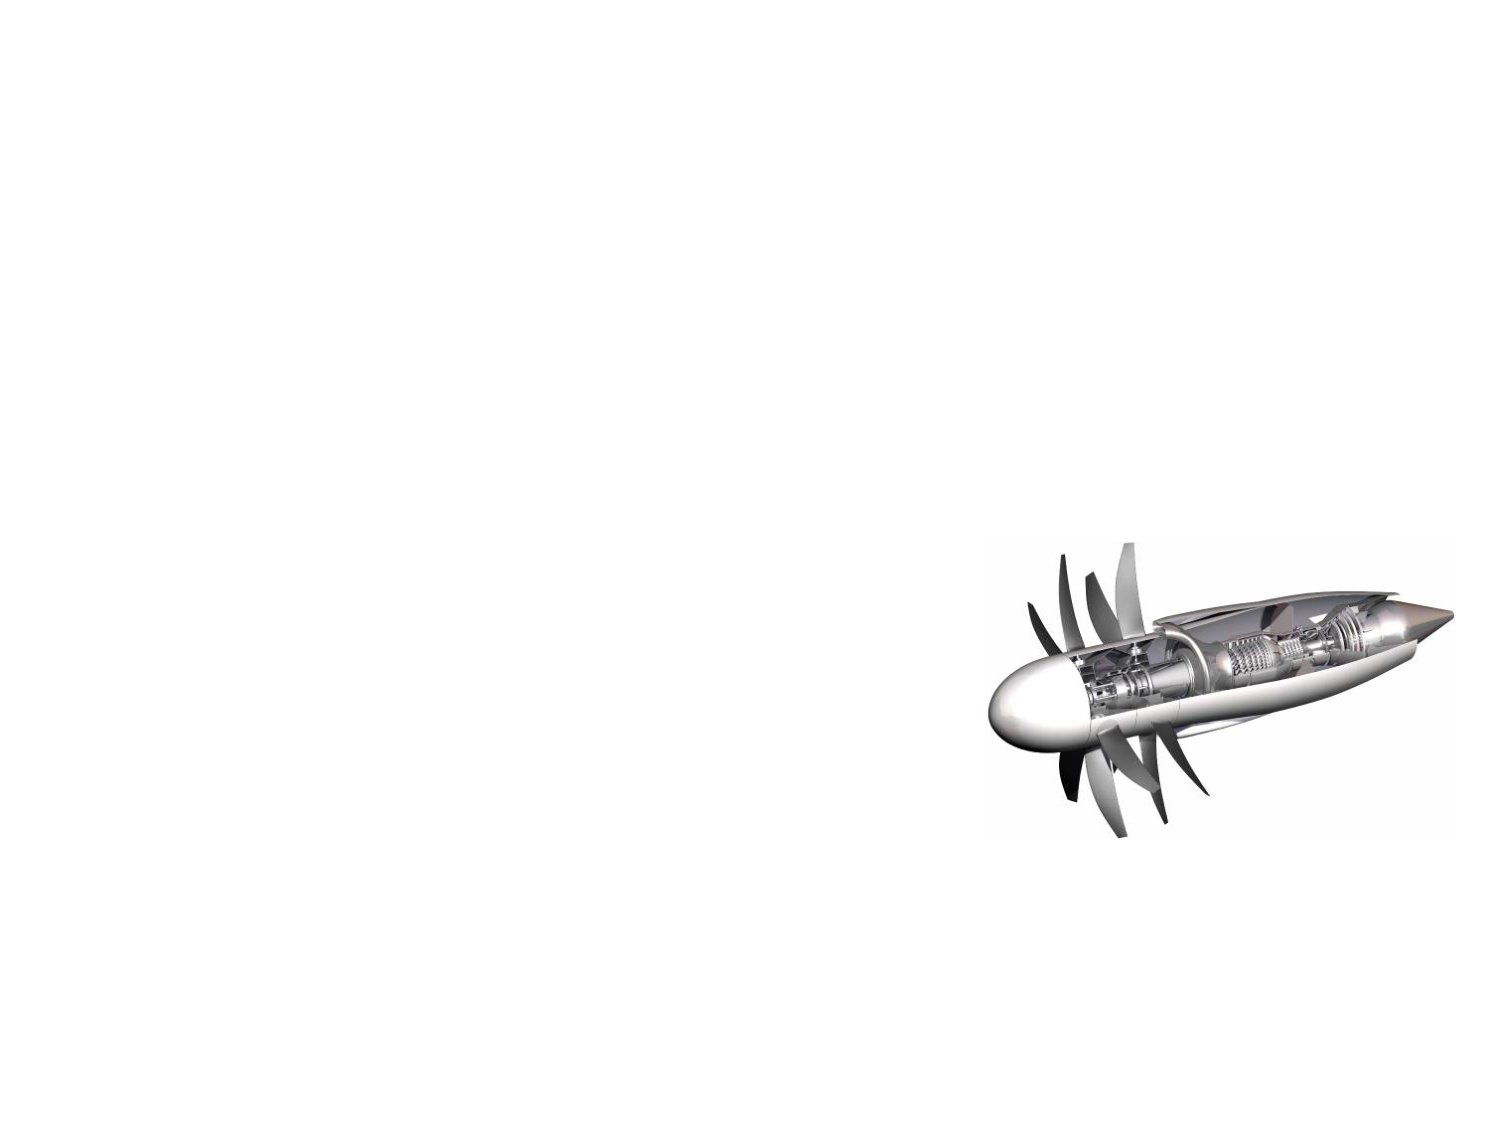
\includegraphics[width=.4\textwidth]{puller.pdf}}
  \subfigure[pusher]{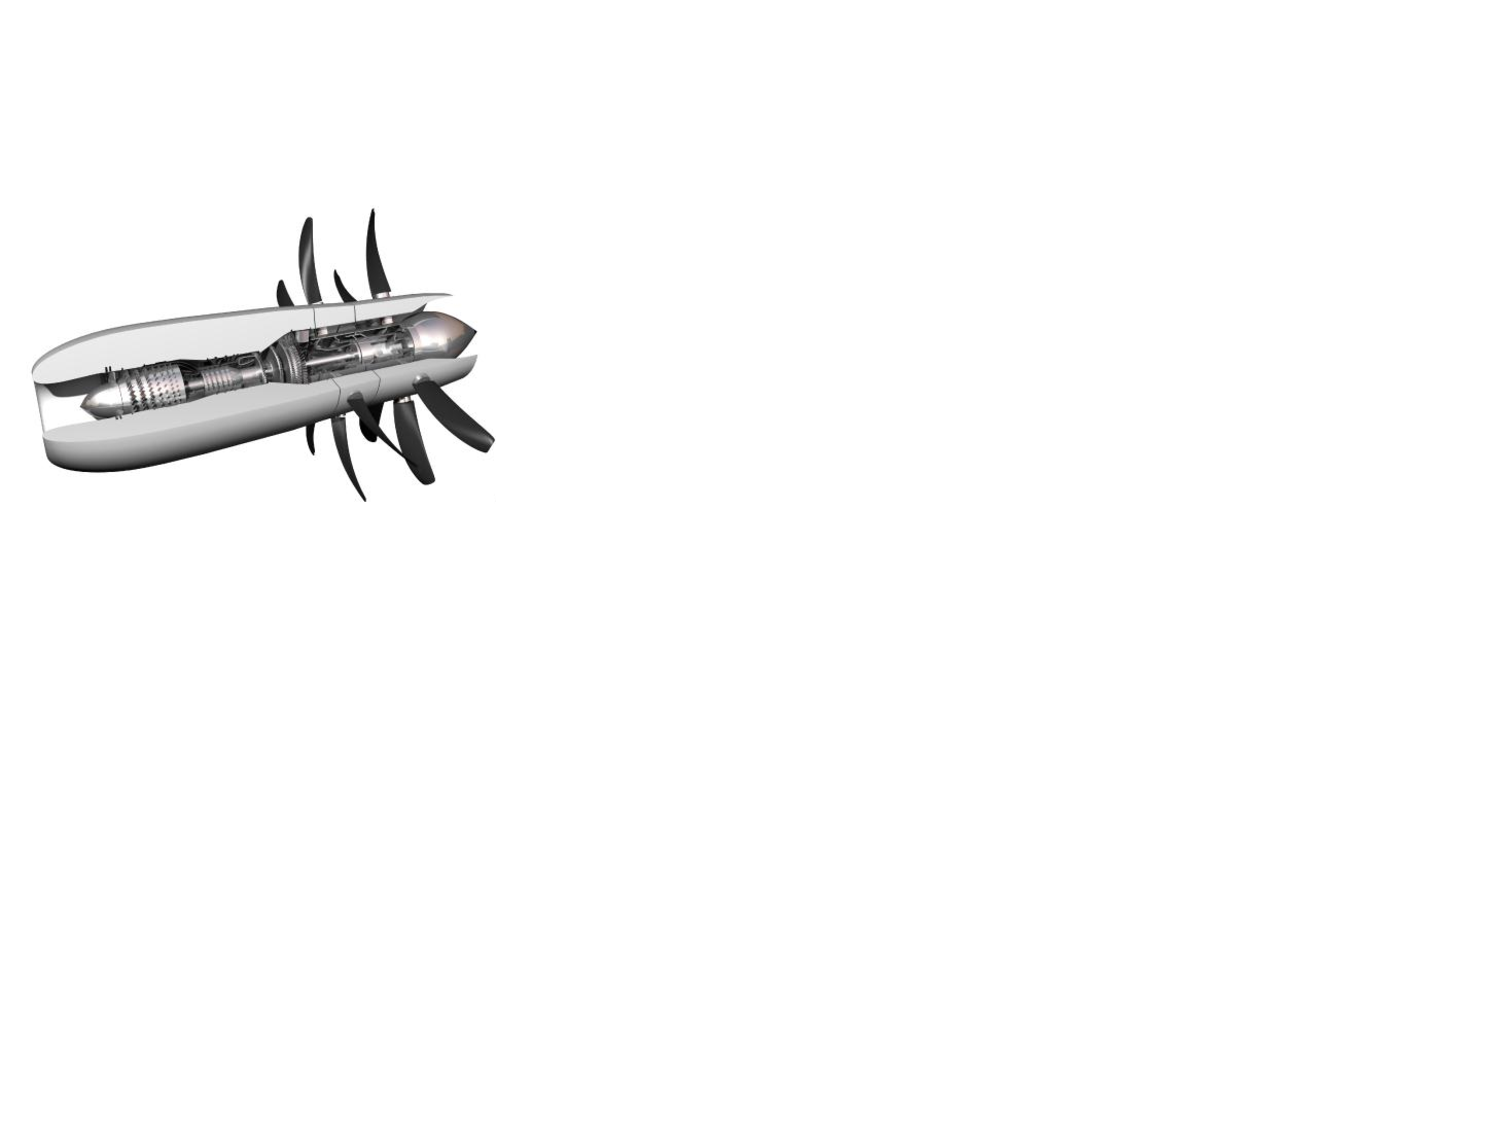
\includegraphics[width=.4\textwidth]{pusher.pdf}}
  \caption{Contra-rotating open rotor configurations, courtesy Rolls-Royce.}
  \label{fig:cror_configurations}
\end{figure}
% For pusher CROR, two types of architectures can be thought:
% one based on a gearbox and the second
% being build around a statorless low-pressure turbine. These
% two 
% \begin{figure}[htp]
%   \centering
%   \subfigure[geared design]{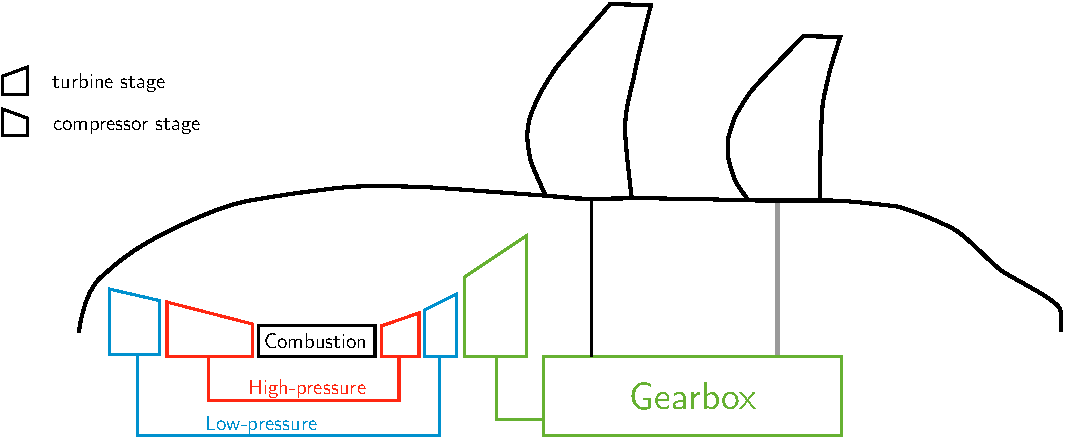
\includegraphics[width=.4\textwidth]{geared_cror.pdf}}
%   \subfigure[statorless low-pressure turbine design]{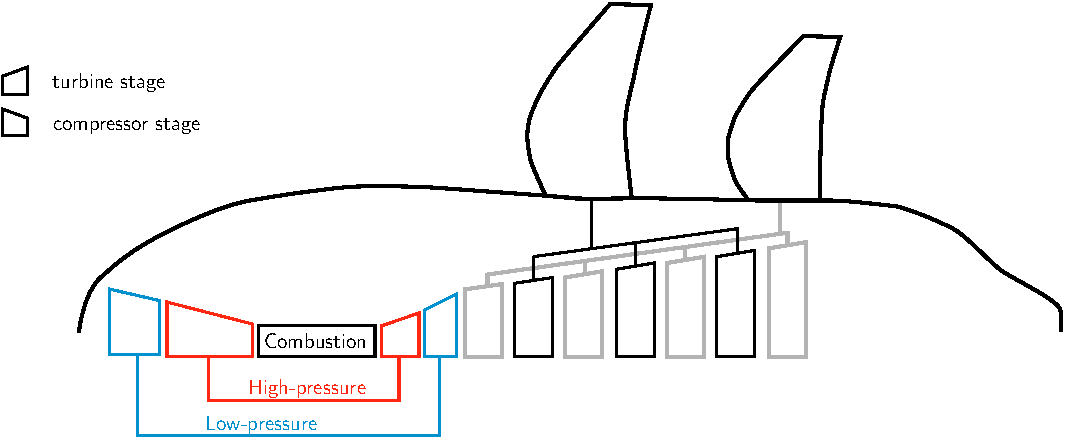
\includegraphics[width=.4\textwidth]{stator_less_cror.pdf}}
%   \caption{Contra-rotating open rotor pusher architectures.}
%   \label{fig:cror_architectures}
% \end{figure}

\subsection{Velocity triangle}
\label{sub:cror_velocity_triangle}
\begin{figure}[htp]
  \centering
  \includegraphics*[scale=0.5]{velocity_triangle_cror.pdf}
  \caption{Velocity triangle applied to a contra-rotating open rotor configuration.}
  \label{fig:velocity_triangle_cror}
\end{figure}
Figure~\ref{fig:velocity_triangle_cror} shows the application
of the velocity triangle to a CROR configuration. The swirl
energy that was lost by the propeller is now used to 
produce more thrust. Therefore, a CROR will finally have a better propulsive
efficiency than a propeller, which explains its study as
a greener engine. In the eighties, 
\citet{Strack1981} and \citet{Hager1988} showed that
using a contra-rotating open rotor technology over
a single propeller gave an increase of $6-8\%$
in propulsive efficiency, explaining its regain of interest.
Today, high-speed propellers blades might lead to higher increase
in efficiency
while keeping a flight Mach number close to $0.8$, enabling its use
for commercial aviation.

\subsection{Similarity coefficients}
\label{sub:cror_similarity_coeff}

In the case of a CROR configuration, the front and the rear rotors 
have to be considered.
Two main ways exist to evaluate the global value of the
similarity coefficients. The first one, chosen by
\citet{Bechet2011} among others, is to consider
that the non-dimensional parameter $D$, $n$ and $J$ are those
of the front rotor for both rotors
\begin{equation}
    J_f = J_r = \frac{V_0}{n_f D_f}, \quad
    C_T = \frac{F_{x_f} + F_{x_r}}{\rho_F n_f ^ 2  D_f ^ 4}, \quad
    C_P = \Omega_f \frac{M_{x_f} + M_{x_r}}{\rho_f n_f ^ 3 D_f ^ 5}, \quad
    \eta = J_f \frac{C_T}{C_P}.
\end{equation} 
The second one uses the non-dimensional parameter of the current rotor,
as done by \citet{Stuermer2008} and \citet{Zachariadis2011}.
The first approach is retained for the current work as it allows
to simplify the comparison of the similarity coefficient with equivalent propellers.


\section{Unsteadinesses}
\label{sec:cror_unsteady}
%!TEX root = ../../../adrien_gomar_phd.tex

\subsection{From steady to unsteady phenomena}
\label{sub:cror_from_steady_to_unsteady_phenomena}

The flow generated behind the front rotor
is steady in its frame of reference. Nevertheless,
due to the relative speed difference between the
front and the rear rotor, these steady flow distortions are
seen as unsteady features by the rear rotor. 
These unsteadiness are correlated to the Blade Passing Frequency (BPF):
\begin{equation}
	f = \frac{\Omega_{rel} B_{opp}}{2 \pi},
\end{equation}
where $\Omega_{rel}$ is the relative speed difference between
the current and the opposite row
and $B_{opp}$ the number of blades in the opposite row.

\subsection{Main unsteadinesses}
\label{sub:cror_main_unsteadinesses}

In sec.~\ref{sub:cror_propeller_physics}, the main physical phenomena
that appears in a propeller have been introduced. As seen above, due to
the relative speed difference between the two rotors, these phenomena
that were steady in their frame of reference are now seen as unsteady features
by the rear rotor. As such, to numerically simulate them, unsteady computations
will be needed. In this aim, the following section will be devoted to the classification
of unsteady phenomena that appears in CROR in 
order to choose an efficient strategy to simulate them.

\paragraph{Tip vortices}

As shown previously in Fig.~\ref{fig:propeller_tip_vortices}, tip vortices are formed
at blade tips due to the pressure difference between each side of the blades.
If nothing particular is done, this low momentum perturbation can
hit the rear rotor and induce large unsteady fluctuations. To avoid this,
the rear rotor blades are clipped as mentioned earlier. 
This unsteadiness is correlated with the BPF.

\paragraph{Wakes and potential effects}

Compared to an isolated rotor, as for the case of a propeller,
the presence of the rear rotor gives rise to an unsteady
interaction by means of potential effects. In addition, wakes generated
behind the front rotor interact with the rear rotor.
This is schematically represented in Fig.~\ref{fig:cror_wakes_potential}.
\begin{figure}[htp]
  \centering
  \includegraphics*[width=0.30\textwidth]{cror_wakes_potential.pdf}
  \caption{Wakes and potential effects in a 
  contra-rotating open rotor configuration.}
  \label{fig:cror_wakes_potential}
\end{figure}
These two phenomena are correlated with the blade passing frequency.
In addition to this, vortex shedding phenomena may occur behind the blades, 
the frequency being not known a priori.
This phenomenon is more likely to appear behind blades with a bluff trailing edge.
This is not a common design in industrial configuration as a bluff trailing edge
gives larger drag. Therefore, we can consider here that 
wake and potential effects are the driving unsteady phenomena.

\paragraph{Non-uniform inflow and installation effects}

In maneuver, the nacelle of the CROR is in incidence with respect to the incoming flow
which results in a non-uniform velocity triangle on the blades.
This leads to in-plane forces. This is an unsteady phenomenon
whose frequency is correlated with the rotation frequency $\Omega / 2 \pi$.
The presence of a pylon (installation effect) give rises to an unsteady frequency
also correlated with the rotation frequency when a pusher CROR is considered.
It is important as it changes the performances and flow behavior around the CROR.


\section{Challenges}
\label{sec:cror_challenges}
%!TEX root = ../../../adrien_gomar_phd.tex

Several challenges are still open for CROR
to become a viable engine for the next generation aircraft.
In this way, we classify and describe each of them in the following sections.

\paragraph{Classification}
Figure~\ref{fig:cror_challenges} depicts current challenges associated
with CROR configurations. Three main fields are involved: aerodynamics,
aeroacoustics and aeroelasticity.
\begin{figure}[htp]
  \centering
  \includegraphics*[scale=0.8]{challenges.pdf}
  \caption{Challenges raised by contra-rotating open rotor configurations.}
  \label{fig:cror_challenges}
\end{figure}

\paragraph{Aerodynamics}
Theoretically, 
the CROR is meant to have a better propulsive efficiency than a turbofan or a
propeller. However, as it is a new architecture, studies need to be conducted
to understand its flow physics. In particular,
aerodynamic interactions between the two rotors need to be better understood.

The research on the aerodynamic of the CRORs is divided in two main
axis: the first axis deals with the design of CRORs while the second
analyzes the unsteady flow physics that develop on given design.

Toward the first axis, 
\citet{Hendricks2011} developed an open-rotor cycle model based
on experimental performance characteristics made at NASA. This is 
an empiric approach that suffers from the impossibility to build new designs.
\citet{Peters2012} developed a similar code to design their CROR. The aeroacoustic
characteristics of the final design is assessed by a 
full annulus unsteady simulation even though the design is 
based on experimental correlations.
To improve the approach to design new CRORs, 
\citet{Bechet2011} used a lifting-line code to
initialize a gradient optimization procedure based on mixing-plane
computations. This led to a gain of almost a half point
in CROR efficiency. This is more general than an empiric strategy
if the mixing-plane computations are reliable to assess the performance
parameters of CROR. 

Toward the second axis, \citet{Zachariadis2011}
compared the performance prediction of mixing plane computations
to experimental data made on an open-rotor test case.
They found a fair agreement for the thrust and power coefficients, however
small discrepancies on the coefficients led to significant errors on their ratio,
\emph{i.e.} the efficiency.
\citet{Vion2011} and \citet{Stuermer2008} used unsteady
CFD computations to assess the unsteady performance and flow features.
\citet{Stuermer2008} and \citet{Francois2013} demonstrated through a code to code comparison
that CFD was mature enough to estimate in-plane forces.

\paragraph{Aeroacoustics}
Lot of research effort is put on the second challenge which
is aeroacoustic since the absence of a duct allows noise generated
by CROR to propagate far away.
In the late eighties, \citet{Hager1988}
conducted at NASA a large project on innovative propulsion systems for the
next generation aircrafts. The potential of the CROR configuration
was identified but the noise emitted was so high that the only way
thought to use such an engine was to put noise liners in the fuselage. This resulted in 
increased weight. Together with the decrease of the price of the
barrel in the late eighties, the CROR never reached the commercial
aviation. This is why, today, a lot of research effort is put on the
understanding and mastering of noise sources in CRORs.
Two main types of noise have been identified: tonal noise which comes from
the interaction of both rotors and is mainly present at low-speed flight conditions 
(namely take-off and landing)
and broadband noise which comes from turbulence and is predominant
at high-speed flight conditions (namely cruise).
Several CFD studies have been performed in the literature.
\citet{Peters2012} showed that unsteady CFD simulation is able
to reproduce the aeroacoustic footprint of a CROR. They then optimized
their CROR and showed that this optimized CROR design may be mature enough
for noise certification. \citet{Hoffer2012} and \citet{Ferrante2013}
developed an efficient CFD approach to simulate the aeroacoustics of CRORs.
It is based on a Fourier-based time method. The approach is able to
account for incidence effects which is particularly interesting
considering that the noise of installed configuration is drastically
different from the isolated one (see \citet{Hager1988}).

\paragraph{Aeroelasticity}
The third challenge is the less studied in the numerical literature.
This why in this thesis, the aeroelasticity of CROR will be assessed.
Two main aeroelastic phenomena have been identified during preliminary studies
during the eighties by \citet{Hager1988}: whirl flutter, \emph{i.e.} the self-excited
movement of the whole nacelle, and blade flutter, \emph{i.e.} the vibration
of the blades.
For a turbofan engine to achieve certification, it must be 
demonstrated that one released fan blade can be safely contained 
within the engine’s fan case as written in the 
Certification Specifications for Engines (CSE) of the EASA:
\begin{quote}
	"It must be demonstrated that any single compressor or turbine blade will be contained after Failure and 
that no Hazardous Engine Effect can arise as a result of other Engine damage likely to occur before 
Engine shut down following a blade Failure"
\end{quote}
In the case of propellers and contra-rotating open rotors, due to the absence of a nacelle,
this can not be done. To achieve certification, it must be demonstrated that the probability of a blade
failure (or any failure) should not exceed $1e^{-8}$ per propeller flight hour as written in 
the Certification Specifications for Propellers (CSP) of the EASA:
\begin{quote}
	"It must be shown that Hazardous Propeller Effects will not occur at a rate in excess of that defined 
as Extremely Remote. The estimated probability for individual failures may be insufficiently precise 
to enable the total rate for Hazardous Propeller Effects to be assessed. For Propeller certification, it 
is acceptable to consider that the intent of this paragraph is achieved if the probability of a 
Hazardous Propeller Effect arising from an individual failure can be predicted to be not greater than 
$1e^{-8}$ per Propeller flight hour. It will also be accepted that, in dealing with probabilities of this low 
order of magnitude, absolute proof is not possible and reliance must be placed on engineering 
judgment and previous experience combined with sound design and test philosophies" 
\end{quote}
This explains why aeroelasticity of contra-rotating open rotors should be assessed.
However, this challenge is less studied in the literature compared to 
aerodynamic or aeroacoustic issues.
To the author knowledge, only whirl flutter has been investigated
in the CROR literature by \citet{CISicot2011a} and 
\citet{Verley2013} and these studies mainly
discuss the simulation tools needed to compute such a phenomenon as
no experimental data are available.



% \chconclu{The main flow physic that develops in contra-rotating open rotors
% has been described. The unsteady phenomena that develops through this
% engine are mostly correlated with the blade passing frequency, except for
% the installation effects and the non-uniform inflow. The challenges
% associated with this type of engine are recalled and it is highlighted 
% that aeroelasticity of such systems remain unstudied. This is
% why the present thesis will focus on aeroelasticity.}
